\begin{frame}{Постановка задачі}
	\manimate
	Користувачі мають 2 матриці розмірів $N \times N$ та хочуть обрахувати їх добуток у розподіленому середовищі.
	Між користувачами виникає конфлікт, оскільки у них спільний, рівноправний та конкурентний доступ до розподіленого середовища. 
\end{frame}

\begin{frame}{Структура Cloud середовища}
	\manimate
	
	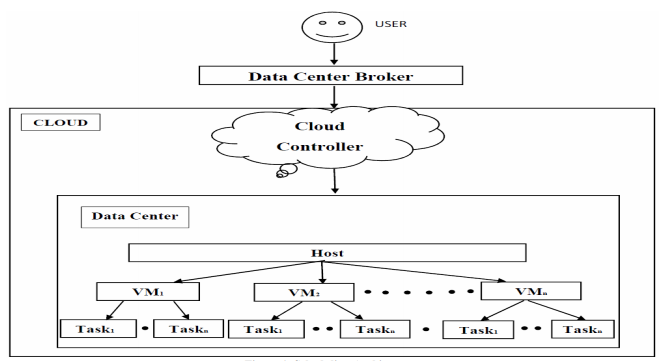
\includegraphics[width=1.0\linewidth]{im/cloud_representation}
\end{frame}

\begin{frame}{Множення матриць блочно}
	\manimate
	Для матриць розмірів $N \times N$ вибирається розмір розрізання $n: n \bigm| N, k = \frac{N}{n}$. Отримуємо $k^2$ задач множення матриць $n \times N$ та $N \times n$.
	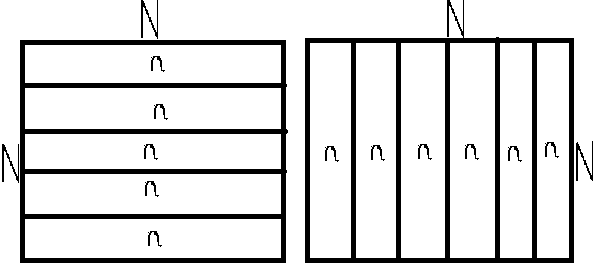
\includegraphics[width=0.8\linewidth]{im/matrixmatrix}
\end{frame}

\begin{frame}{Ігрова постановка задачі}
\manimate
	Гра двох користувачів:
	\begin{itemize}
		\item[1.] Користувачі вибирають розбиття $n_1, n_2$.
		\item[2.] Користувачі розрізають матриці, формують задачі та надсилають їх до хмари.
		\item[3.] Користувачі отримують результати.
	\end{itemize}
	Часом для користувача вважається час отримання усіх результатів надісланих задач.
\end{frame}

\begin{frame}{Ігрова постановка задачі}
\manimate
	Таким чином отримано біматричну гру з матрицями програшів $(A,B)$.
\end{frame}